\documentclass{article}
\usepackage[a4paper, total={7in, 10in}]{geometry}
\usepackage{fancyhdr}
\usepackage{pdfpages}

\title{How to write a scientific article}
\author{
    Hyosang Kang\\
    \small Division of Mathematics\\ 
    \small School of Interdisciplinary Studies\\ 
    \small DGIST
}
\date{
    July 21, 2023\\ 
    \small Jeonbuk Science High School
}

\fancyhf{}
\fancyfoot[R]{\thepage}

\begin{document}

\maketitle
\thispagestyle{fancy}

\section{Introduction}

% what is a scientific article
A scientific article is a written document that often describes the process, results, and conclusions of a scientific research. 
It is a way to publicize your research output and communicate within the scientific community. 
% what is a scientific writing
A scientific writing is a skill for writing a scientific article.
A scientific article is usually written in a format of a journal paper which requires a specific structure and style.
% why we discuss about scientific writing
In this document, we will discuss about how to write a scientific article properly.
We will also discuss how scientific writing should be done with hand-on examples.
At the end of our discussion, you will understand a good scientific writing skill helps not only producing a good scientific article, but also accomplishing a successful research. 

% who are the potential audiences
This document is designed for a special lecture to students who begin to write their first scientific article.
The author assumes the range of audiences are from senior high school students to undergraduate students, specifically in South Korea.
% why am I write this document in English
By the way, you may wonder why this document is written in English.
First, most of scientific articles are written in English, so you must get used to English writing whether you like it or not.
Second, a tranlating Korean contents to English is not a good way of writing a scientific article, because there is no one-to-one mapping between Korean and English. You will end up with either an awkward English translation or rewriting the whole contents in English from scratch.



\section{Let's group up before we start}

% group up
Before we start, let's group up by three (or four) people.
Each group will have a writer, a reporter, and a interpreter.
There may be two interpreter depending on the size of your group.
% the roles of the group members
The group members should actively participate in the discussion of the topics in the following sections.
The writer will write down the conclusion of the group in this piece of paper.
The reporter will report the conclusion of the group to the class when called by the lecturer.
The interpreter will rephrase, elaborate, criticize, or summarize the arguments in the group.
% attach sticker to the reporter
Once you have decided the roles of the group members, please attach a sticker to the chest of the reporter so that the lecturer can see who is the reporter in the group.


\newpage
\section{Sections of a scientific article}

% sections of a scientific article
Every scientific article is composed of several sections.
Sections are organized in a way that the reader can easily follow the context of the article.
Using sections, the writer can also easily organize the contents of the article.
Let's discuss about what kinds of sections are there.
% sample scientific articles
In the appendix, you can find two sample scientific articles listed below:
\begin{itemize}
    \item \textbf{Brunton S.L. et al.} (2016) Discovering governing equations from data by sparse identification of nonlinear dynamical systems. PNAS, 113(15), 3932-3937.
    \item \textbf{Rivest R.L. et al.} (1978) A method for obtaining digital signatures and public-key cryptosystems. Communications of the ACM, 21(2), 120-126.
\end{itemize}
You should not attempt to read the whole document.
Instead, quickly skim through the document and try to distinguish the sections in the contents.
While doing so, try to name the sections. (e.g. Abstract, Introduction, Method, Results, Conclusion, etc.) 
% discuss and conclude about sections
Here is the list of questions you should discuss in your group:
\begin{enumerate}
    \item What are names of sections (not the titles!) you have found in two sample articles? 
    \vspace{2in}
    \item What do you think the role of each section is?
    \vspace{2in}
    \item What are the sections in common from two sample articles?
    \vspace{2in}
    \item What are the differences in the organization of sections in two sample articles?
    \vspace{2in}
\end{enumerate}


\newpage
\section{The order of writing the sections}

% in the beginning of writing
Now suppose you are about to write a scientific article from scratch.
You opened your favorite text editor and are ready to write the first sentence.
What should you write first?
% discuss order of writing
Here is the list of questions you should discuss in your group:
\begin{enumerate}
    \item From the list of sections you have found previously, what section should you write first, and why?
    \vspace{2in}
    \item In what order would you write the rest of the sections, and why?
    \vspace{2in}
    \item In which section, would you spend most of your time in writing and why?
    \vspace{2in}
\end{enumerate}


\newpage
\section{What, why, and how}

% every sentence in a scientific article is an answer for an either what, why, or how question
When we make a scientific argument, we have a concrete form of a question in our mind, and this question is either what, why, or how question.
A what question is something like: What is \textit{thing} that we are going to talking about? What is the problem about that \textit{thing}? What have people done about that \textit{thing}?
A why question is something like: Why is studying that \textit{thing} important? Why is solving our problem important? Why is that our problem difficult to solve?
A how question is something like: How are we going to solve our problem? How are we going to prove that our solution is correct? How are we going to evaluate our solution?

% writing is a consequence of answering a logical flow of questions
Writing is a dialogue between the writer and the reader.
Thus writer should keep the readers focused by laying out a series of answers to the questions that the reader might have in mind while reading the document.
In the scientific writing, authors should clearly set the level of the audience so that they can project the questions onto their audience properly.
Once the questions are properly projected, the rest of the work is to write a truthful, factual, objective, and comprehensive answers to the questions.

% classify the sentences in the sample articles
Let's do an exercise to classify the sentences in the sample articles into answers to what, why, and how questions.
\begin{enumerate}
    \item Divide the sentences in the sample articles into three groups: what, why, and how.
    \begin{itemize}
        \item From the \underline{first page} of \textbf{Brunton S.L. et al.} (2016)\\
    \fbox{\parbox{.8\textwidth}{
    Advances in machine learning (Ref. \#1) and data science (Ref. \#22) have promised a renaissance in the analysis and understanding of complex data, extracting patterns in vast multimodal data that are beyond the ability of humans to grasp. 
    However, despite the rapid development of tools to understand static data based on statistical relationships, there has been slow progress in distilling physical models of dynamic processes from big data. 
    This has limited the ability of data science models to extrapolate the dynamics beyond the attractor where they were sampled and constructed.}}
        \item From the \underline{first page} of \textbf{Rivest R.L. et al.} (1978)\\
    \fbox{\parbox{.8\textwidth}{
    An encryption (or decryption) procedure typically consists of a general method and an encryption key. 
    The general method, under control of the key, enciphers a message M to obtain the enciphered form of the message, called the ciphertext C. 
    Everyone can use the same general method; the security of a given procedure will rest on the security of the key. 
    Revealing an encryption algorithm then means revealing the key.}}
    \end{itemize}
    \item Write down a concrete question for each sentence that the sentence is the answer for.
    \begin{itemize}
        \item Advances in machine learning (Ref. \#1) and data science (Ref. \#22) have promised a renaissance in the analysis and understanding of complex data, extracting patterns in vast multimodal data that are beyond the ability of humans to grasp. 
        \vspace{1in}
        % What practices that the machine learning and data science have been contributed?
        \item However, despite the rapid development of tools to understand static data based on statistical relationships, there has been slow progress in distilling physical models of dynamic processes from big data. 
        \vspace{1in}
        % What areas of studies on big data have a problem? What is the problem? Why is that problem important?
        \item This has limited the ability of data science models to extrapolate the dynamics beyond the attractor where they were sampled and constructed. 
        \vspace{1in}
        % What is the consequence of the problem being unsolved?
    \end{itemize}
    \item (Homework) Do the same with the sentences in the second box above.
\end{enumerate}



% few tips for improving your scientific writing skill
\section{Few tips}
Here are some tips for improving your scientific writing skill.
\begin{enumerate}
    \item Give a plenty of time to write, and also for the revision. Start writing at the beginning of your research, not at the end.
    \item Make a claim only with a concrete logical argument, or with a credible reference (for example, wiki is \underline{not} a credible source.)
    \item Avoid using any subjective adjectives (e.g. important, significant, etc.) or adverbs (e.g. very, extremely, highly, etc.)
    \item Remove redundencies in your sentences, paragraphs, and sections. (Unfortunately, creating redundancy is what text-generating AIs are extremely good at! So do not rely on them too much.)
    \item Use as many writing assistant tools as possible (e.g. spell checker, grammar checker, etc.) Learn how to use \LaTeX (pronounced as ``lay-tech'') or any other word processor that supports mathematical equations. Hangul\textsuperscript{\textregistered} is unaccepted as an official word processor in world standard.
\end{enumerate}

\section{Wrapping up}
Before we finish, let's discuss about the following things among your group members:
\begin{enumerate}
    \item What have you learned from today's lecture?
    \vspace{2in}
    \item What was the thing that highlighted you the most, and why do you think so?
    \vspace{2in}
    \item What would you do differently in your scientific writing than you thought to do (or already have been doing) before this lecture?
    \vspace{2in}
\end{enumerate}

\newpage
\*
\newpage

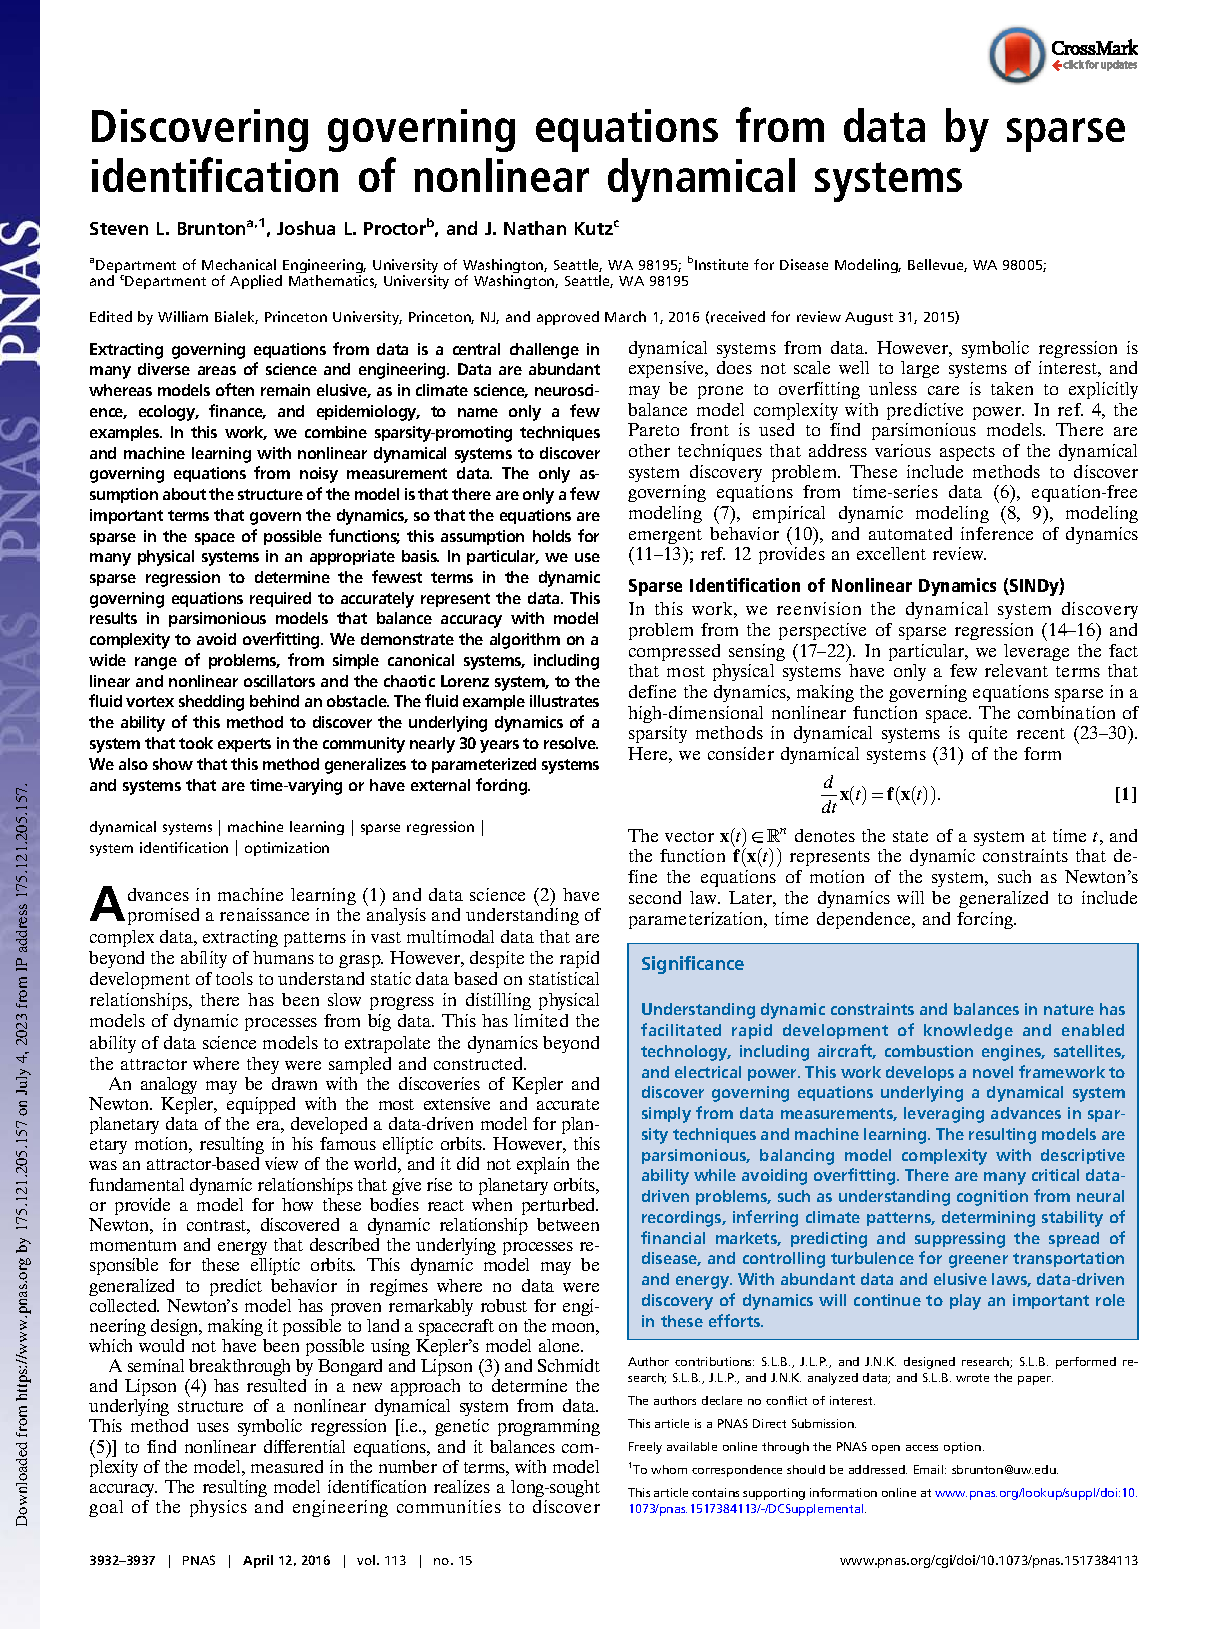
\includepdf[pages=-]{sample-1.pdf}
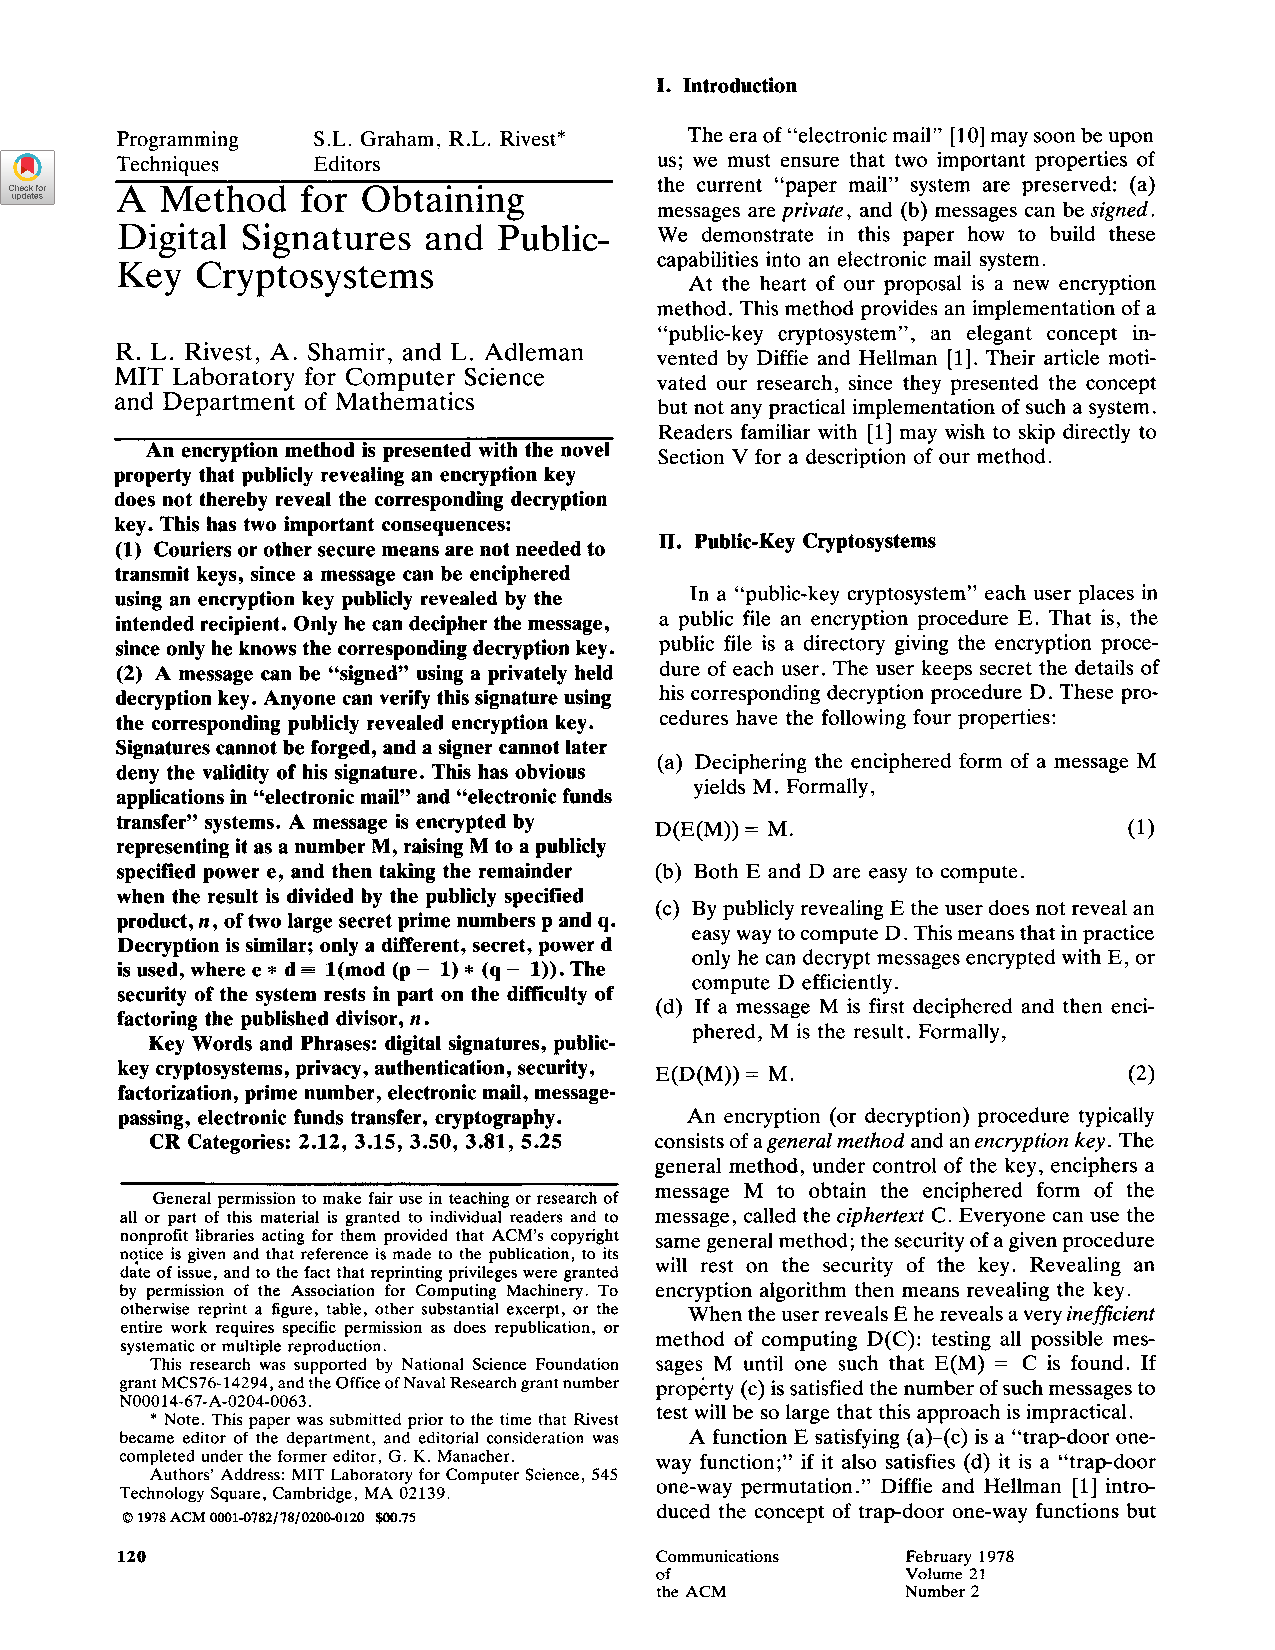
\includepdf[pages=-]{sample-2.pdf}

\end{document}